\documentclass[10pt]{article}
\usepackage{hyperref}
\usepackage{amsmath}
\usepackage{tikz}
\usepackage[margin=1in]{geometry}
\usetikzlibrary{arrows,calc}
\usepackage{biblatex}
\addbibresource{./references.bib}
\begin{document}
%
\section{Linear Quadrilateral (2D)}
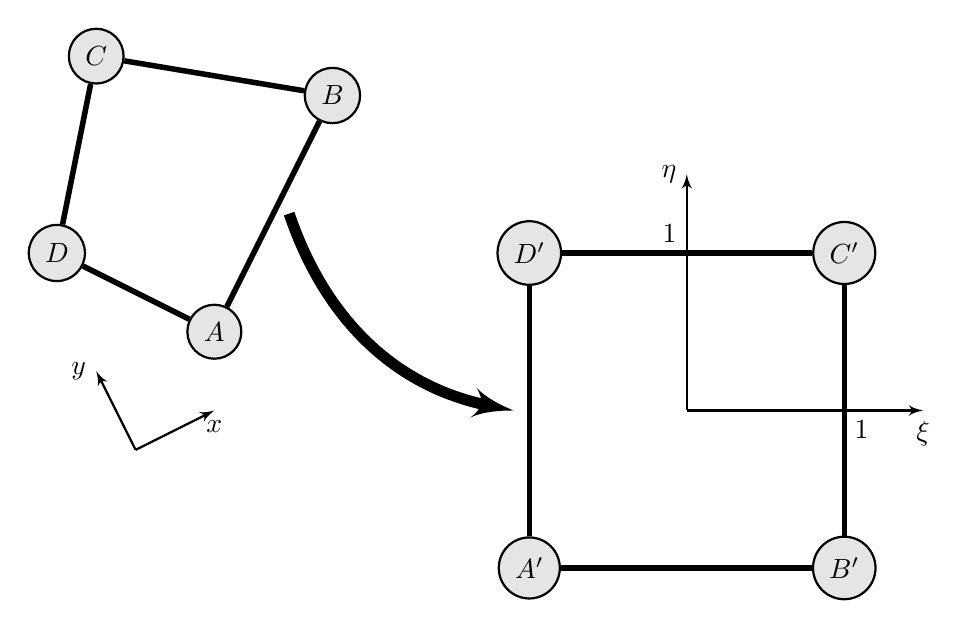
\begin{tikzpicture}[>=latex',thick]
    \tikzstyle{n}=[circle, draw=black, minimum size=0.5cm, fill=black!10]

    \node[n] (Ao) at (-6cm, 1cm) {$A$};
    \node[n] (Co) at (-7.5cm, 4.5cm) {$C$};
    \node[n] (Do) at (-8cm, 2cm) {$D$};
    \node[n] (Bo) at (-4.5cm, 4cm) {$B$};
    \draw (Ao) edge[line width=2pt] (Bo);
    \draw (Bo) edge[line width=2pt] (Co);
    \draw (Co) edge[line width=2pt] (Do);
    \draw (Do) edge[line width=2pt] (Ao);

    \draw (-7cm, -0.5cm) edge[->] node[pos=1.0, below] {$x$} (-6cm, 0cm);
    \draw (-7cm, -0.5cm) edge[->] node[pos=1.0, left] {$y$} (-7.5cm, 0.5cm);

    \coordinate (Xm) at (3cm, 0);
    \coordinate (Ym) at (0, 3cm);
    \coordinate (origin) at (0,0);

    \node[n] (B) at (2cm, -2cm) {$B'$};
    \node[n] (C) at (2cm, 2cm) {$C'$};
    \node[n] (D) at (-2cm, 2cm) {$D'$};
    \node[n] (A) at (-2cm, -2cm) {$A'$};

    \node[above left] at (0, 2cm) {$1$};
    \node[below right] at (2cm, 0) {$1$};

    \draw ($0.5*(Ao) + 0.5*(Bo) + (0.2cm,0)$) edge[bend right, ->,line width=4pt] ($0.5*(D) + 0.5*(A) + (-0.2cm, 0)$);
    
    \draw (A) edge[line width=2pt] (B);
    \draw (B) edge[line width=2pt] (C);
    \draw (C) edge[line width=2pt] (D);
    \draw (D) edge[line width=2pt] (A);
    \draw (origin) edge[->] node[pos=1.0, below] {$\xi$} (Xm);
    \draw (origin) edge[->] node[pos=1.0, left] {$\eta$} (Ym);
\end{tikzpicture}

\begin{itemize}
    \item Local to global coordinates:
        \begin{align}
            \begin{bmatrix}
                x \\
                y \\
                1
            \end{bmatrix}
            &=
            \begin{bmatrix}
                A_x & B_x & C_x & D_x \\
                A_y & B_y & C_y & D_y \\
                1 & 1 & 1 & 1
            \end{bmatrix} 
            \begin{bmatrix}
                N_A \\
                N_B \\
                N_C \\
                N_D
            \end{bmatrix} \\
            \begin{bmatrix}
                x \\
                y 
            \end{bmatrix}
            &=
            \frac{1}{4}
            \begin{bmatrix}
                A_x & B_x & C_x & D_x \\
                A_y & B_y & C_y & D_y
            \end{bmatrix} 
            \begin{bmatrix}
                (1 - \xi)(1 - \eta) \\
                (1 + \xi)(1 - \eta) \\
                (1 + \xi)(1 + \eta) \\
                (1 - \xi)(1 + \eta) 
            \end{bmatrix}
        \end{align}
    \item Jacobian:
        \begin{align}
            \begin{bmatrix}
                U_x & U_y \\
                V_x & V_y \\
                W_x & W_y \\
            \end{bmatrix}
            &=
            \begin{bmatrix}
                1 & -1 & 1 & -1 \\
                -1 & 1 & 1 & -1 \\
                -1 & -1 & 1 & 1
            \end{bmatrix}
            \begin{bmatrix}
                A_x & A_y \\
                B_x & B_y \\
                C_x & C_y \\
                D_x & D_y
            \end{bmatrix}
            \\
            \mathbf{J} &= \frac{\partial \mathbf{x}}{\partial \boldsymbol{\xi}}
            =
            \begin{bmatrix}
                \frac{\partial x}{\partial \xi} & \frac{\partial x}{\partial \xi} \\
                \frac{\partial y}{\partial \eta} & \frac{\partial y}{\partial \eta}
            \end{bmatrix}
            =
            \frac{1}{4}
            \begin{bmatrix}
                U_x \eta + V_x & U_x \xi + W_x \\
                U_y \eta + V_y & U_y \xi + W_y \\
            \end{bmatrix} \\
            \det \mathbf{J}
            &=
            \frac{1}{16} ({\left(U_{x} \eta + V_{x}\right)} {\left(U_{y} \xi + W_{y}\right)}
                - {\left(U_{y} \eta + V_{y}\right)} {\left(U_{x} \xi + W_{x}\right)})
        \end{align}
    \item Shape functions:
        \begin{align}
            \mathbf{N}
            &=
            \begin{bmatrix}
                N_A \\
                N_B \\
                N_C \\
                N_D
            \end{bmatrix}
            =
            \frac{1}{4}
            \begin{bmatrix}
                (1 - \xi)(1 - \eta) \\
                (1 + \xi)(1 - \eta) \\
                (1 + \xi)(1 + \eta) \\
                (1 - \xi)(1 + \eta) 
            \end{bmatrix}
        \end{align}
    \item Gradient of shape functions:
        \begin{align}
            \frac{\partial \mathbf{N}}{\partial \mathbf{x}}
            &=
            \begin{bmatrix}
                \frac{\partial N_A}{\partial x} & \frac{\partial N_A}{\partial y} \\
                \frac{\partial N_B}{\partial x} & \frac{\partial N_B}{\partial y} \\
                \frac{\partial N_C}{\partial x} & \frac{\partial N_C}{\partial y} \\
                \frac{\partial N_D}{\partial x} & \frac{\partial N_D}{\partial y}
            \end{bmatrix}
            =
            \begin{bmatrix}
                \frac{\partial N_A}{\partial \xi} & \frac{\partial N_A}{\partial \eta} \\
                \frac{\partial N_B}{\partial \xi} & \frac{\partial N_B}{\partial \eta} \\
                \frac{\partial N_C}{\partial \xi} & \frac{\partial N_C}{\partial \eta} \\
                \frac{\partial N_D}{\partial \xi} & \frac{\partial N_D}{\partial \eta}
            \end{bmatrix}
            \begin{bmatrix}
                \frac{\partial \xi}{\partial x} & \frac{\partial \xi}{\partial y} \\
                \frac{\partial \eta}{\partial x} & \frac{\partial \eta}{\partial y}
            \end{bmatrix} \\
            \frac{\partial \mathbf{N}}{\partial \mathbf{x}}
            &=
            \frac{1}{16 \det \mathbf{J}}
            \begin{bmatrix}
                -(1-\eta) & -(1-\xi) \\
                1-\eta & -(1+\xi \\
                1+\eta & 1+\xi \\
                -(1+\eta) & 1-\xi
            \end{bmatrix}
            \begin{bmatrix}
                U_y \xi + W_y & -(U_x \xi + W_x) \\
                -(U_y \eta + V_y) & U_x \eta + V_x \\
            \end{bmatrix}
        \end{align}
    \item Global to local coordinates reproduced from \textcite{hua90}:
        \begin{align}
            \begin{bmatrix}
                U_x & U_y \\
                V_x & V_y \\
                W_x & W_y \\
                S_x & S_y
            \end{bmatrix}
            &=
            \begin{bmatrix}
                1 & -1 & 1 & -1 \\
                -1 & 1 & 1 & -1 \\
                -1 & -1 & 1 & 1 \\
                1 & 1 & 1 & 1
            \end{bmatrix}
            \begin{bmatrix}
                A_x & A_y \\
                B_x & B_y \\
                C_x & C_y \\
                D_x & D_y
            \end{bmatrix}
            \\
            \begin{bmatrix}
                S^*_x \\
                S^*_y
            \end{bmatrix}
            &=
            \begin{bmatrix}
                4 x - S_x \\
                4 y - S_y
            \end{bmatrix}
        \end{align}
        Note that except for $S^*_x$ and $S^*_y$, these quantities are the same as used in the jacobian calculation and can be precomputed for the element.

        Using notation from \textcite{hua90}, $r_s = \det \begin{bmatrix} r_x & s_x \\ r_y & s_y \end{bmatrix} = r_x s_y - s_x r_y $.

        Cases:
        \begin{align}
            \begin{bmatrix}
                \xi \\
                \eta
            \end{bmatrix}
            &=
            \begin{cases}
                \begin{bmatrix}
                    A \\
                    (U_{S^*} + V_U \xi) / U_W
                \end{bmatrix} & \mbox{if } U_x U_y U_V U_W \ne 0
            \end{cases}
        \end{align}

\end{itemize}
\printbibliography
\end{document}
